\PassOptionsToPackage{unicode=true}{hyperref} % options for packages loaded elsewhere
\PassOptionsToPackage{hyphens}{url}
%
\documentclass[]{article}
\usepackage{lmodern}
\usepackage{amssymb,amsmath}
\usepackage{ifxetex,ifluatex}
\usepackage{fixltx2e} % provides \textsubscript
\ifnum 0\ifxetex 1\fi\ifluatex 1\fi=0 % if pdftex
  \usepackage[T1]{fontenc}
  \usepackage[utf8]{inputenc}
  \usepackage{textcomp} % provides euro and other symbols
\else % if luatex or xelatex
  \usepackage{unicode-math}
  \defaultfontfeatures{Ligatures=TeX,Scale=MatchLowercase}
\fi
% use upquote if available, for straight quotes in verbatim environments
\IfFileExists{upquote.sty}{\usepackage{upquote}}{}
% use microtype if available
\IfFileExists{microtype.sty}{%
\usepackage[]{microtype}
\UseMicrotypeSet[protrusion]{basicmath} % disable protrusion for tt fonts
}{}
\IfFileExists{parskip.sty}{%
\usepackage{parskip}
}{% else
\setlength{\parindent}{0pt}
\setlength{\parskip}{6pt plus 2pt minus 1pt}
}
\usepackage{hyperref}
\hypersetup{
            pdftitle={ESM204 Assignment 3},
            pdfauthor={Simone Albuquerque, Claudia Flores, and Anthony Luna},
            pdfborder={0 0 0},
            breaklinks=true}
\urlstyle{same}  % don't use monospace font for urls
\usepackage[margin=1in]{geometry}
\usepackage{color}
\usepackage{fancyvrb}
\newcommand{\VerbBar}{|}
\newcommand{\VERB}{\Verb[commandchars=\\\{\}]}
\DefineVerbatimEnvironment{Highlighting}{Verbatim}{commandchars=\\\{\}}
% Add ',fontsize=\small' for more characters per line
\usepackage{framed}
\definecolor{shadecolor}{RGB}{248,248,248}
\newenvironment{Shaded}{\begin{snugshade}}{\end{snugshade}}
\newcommand{\AlertTok}[1]{\textcolor[rgb]{0.94,0.16,0.16}{#1}}
\newcommand{\AnnotationTok}[1]{\textcolor[rgb]{0.56,0.35,0.01}{\textbf{\textit{#1}}}}
\newcommand{\AttributeTok}[1]{\textcolor[rgb]{0.77,0.63,0.00}{#1}}
\newcommand{\BaseNTok}[1]{\textcolor[rgb]{0.00,0.00,0.81}{#1}}
\newcommand{\BuiltInTok}[1]{#1}
\newcommand{\CharTok}[1]{\textcolor[rgb]{0.31,0.60,0.02}{#1}}
\newcommand{\CommentTok}[1]{\textcolor[rgb]{0.56,0.35,0.01}{\textit{#1}}}
\newcommand{\CommentVarTok}[1]{\textcolor[rgb]{0.56,0.35,0.01}{\textbf{\textit{#1}}}}
\newcommand{\ConstantTok}[1]{\textcolor[rgb]{0.00,0.00,0.00}{#1}}
\newcommand{\ControlFlowTok}[1]{\textcolor[rgb]{0.13,0.29,0.53}{\textbf{#1}}}
\newcommand{\DataTypeTok}[1]{\textcolor[rgb]{0.13,0.29,0.53}{#1}}
\newcommand{\DecValTok}[1]{\textcolor[rgb]{0.00,0.00,0.81}{#1}}
\newcommand{\DocumentationTok}[1]{\textcolor[rgb]{0.56,0.35,0.01}{\textbf{\textit{#1}}}}
\newcommand{\ErrorTok}[1]{\textcolor[rgb]{0.64,0.00,0.00}{\textbf{#1}}}
\newcommand{\ExtensionTok}[1]{#1}
\newcommand{\FloatTok}[1]{\textcolor[rgb]{0.00,0.00,0.81}{#1}}
\newcommand{\FunctionTok}[1]{\textcolor[rgb]{0.00,0.00,0.00}{#1}}
\newcommand{\ImportTok}[1]{#1}
\newcommand{\InformationTok}[1]{\textcolor[rgb]{0.56,0.35,0.01}{\textbf{\textit{#1}}}}
\newcommand{\KeywordTok}[1]{\textcolor[rgb]{0.13,0.29,0.53}{\textbf{#1}}}
\newcommand{\NormalTok}[1]{#1}
\newcommand{\OperatorTok}[1]{\textcolor[rgb]{0.81,0.36,0.00}{\textbf{#1}}}
\newcommand{\OtherTok}[1]{\textcolor[rgb]{0.56,0.35,0.01}{#1}}
\newcommand{\PreprocessorTok}[1]{\textcolor[rgb]{0.56,0.35,0.01}{\textit{#1}}}
\newcommand{\RegionMarkerTok}[1]{#1}
\newcommand{\SpecialCharTok}[1]{\textcolor[rgb]{0.00,0.00,0.00}{#1}}
\newcommand{\SpecialStringTok}[1]{\textcolor[rgb]{0.31,0.60,0.02}{#1}}
\newcommand{\StringTok}[1]{\textcolor[rgb]{0.31,0.60,0.02}{#1}}
\newcommand{\VariableTok}[1]{\textcolor[rgb]{0.00,0.00,0.00}{#1}}
\newcommand{\VerbatimStringTok}[1]{\textcolor[rgb]{0.31,0.60,0.02}{#1}}
\newcommand{\WarningTok}[1]{\textcolor[rgb]{0.56,0.35,0.01}{\textbf{\textit{#1}}}}
\usepackage{graphicx,grffile}
\makeatletter
\def\maxwidth{\ifdim\Gin@nat@width>\linewidth\linewidth\else\Gin@nat@width\fi}
\def\maxheight{\ifdim\Gin@nat@height>\textheight\textheight\else\Gin@nat@height\fi}
\makeatother
% Scale images if necessary, so that they will not overflow the page
% margins by default, and it is still possible to overwrite the defaults
% using explicit options in \includegraphics[width, height, ...]{}
\setkeys{Gin}{width=\maxwidth,height=\maxheight,keepaspectratio}
\setlength{\emergencystretch}{3em}  % prevent overfull lines
\providecommand{\tightlist}{%
  \setlength{\itemsep}{0pt}\setlength{\parskip}{0pt}}
\setcounter{secnumdepth}{0}
% Redefines (sub)paragraphs to behave more like sections
\ifx\paragraph\undefined\else
\let\oldparagraph\paragraph
\renewcommand{\paragraph}[1]{\oldparagraph{#1}\mbox{}}
\fi
\ifx\subparagraph\undefined\else
\let\oldsubparagraph\subparagraph
\renewcommand{\subparagraph}[1]{\oldsubparagraph{#1}\mbox{}}
\fi

% set default figure placement to htbp
\makeatletter
\def\fps@figure{htbp}
\makeatother


\title{ESM204 Assignment 3}
\author{Simone Albuquerque, Claudia Flores, and Anthony Luna}
\date{}

\begin{document}
\maketitle

\begin{Shaded}
\begin{Highlighting}[]
\CommentTok{#readin Data}
\NormalTok{cost_gas_data<-}\StringTok{ }\KeywordTok{read_csv}\NormalTok{(}\StringTok{"assign_3_data.csv"}\NormalTok{) }\OperatorTok\StringTok{ }
\StringTok{  }\KeywordTok{clean_names}\NormalTok{()}
\end{Highlighting}
\end{Shaded}

\begin{Shaded}
\begin{Highlighting}[]
\CommentTok{# Linear Regression Low Cost Consumer }
\NormalTok{lm_low <-}\StringTok{ }\KeywordTok{lm}\NormalTok{(price_dollars }\OperatorTok{~}\StringTok{ }\NormalTok{q_low_gallons, }\DataTypeTok{data=}\NormalTok{cost_gas_data) }
\CommentTok{#print(lm_low)  #  1.169e+01 + -6.611e-05*q}
\CommentTok{# Linear Regression High Cost Consumer}
\NormalTok{lm_high <-}\StringTok{ }\KeywordTok{lm}\NormalTok{(price_dollars }\OperatorTok{~}\StringTok{ }\NormalTok{q_high_gallons, }\DataTypeTok{data=}\NormalTok{cost_gas_data) }
\CommentTok{#print(lm_high)  #  1.580e+01 + -2.731e-05*q}
\CommentTok{# Linear Regression Aggregate Cost Consumer}
\NormalTok{lm_agg <-}\StringTok{ }\KeywordTok{lm}\NormalTok{(price_dollars }\OperatorTok{~}\StringTok{ }\NormalTok{q_aggregrate, }\DataTypeTok{data=}\NormalTok{cost_gas_data) }
\CommentTok{#print(lm_agg)  #  1.500e+01 + -2.043e-05*q}
\end{Highlighting}
\end{Shaded}

\begin{Shaded}
\begin{Highlighting}[]
\CommentTok{# Demand Curve Coefficients based on linear models}
\NormalTok{I1<-}\StringTok{  }\NormalTok{lm_low}\OperatorTok{$}\NormalTok{coefficients[}\DecValTok{1}\NormalTok{] }
\NormalTok{I2<-}\StringTok{  }\NormalTok{lm_high}\OperatorTok{$}\NormalTok{coefficients[}\DecValTok{1}\NormalTok{]}
\NormalTok{S1<-}\StringTok{  }\NormalTok{lm_low}\OperatorTok{$}\NormalTok{coefficients[}\DecValTok{2}\NormalTok{]}
\NormalTok{S2<-}\StringTok{  }\NormalTok{lm_high}\OperatorTok{$}\NormalTok{coefficients[}\DecValTok{2}\NormalTok{]}

\CommentTok{# functional definition of high and low demand based on linear model}
\NormalTok{low_demand <-}\StringTok{ }\ControlFlowTok{function}\NormalTok{(q)  I1 }\OperatorTok{+}\StringTok{ }\NormalTok{(S1}\OperatorTok{*}\NormalTok{q)}
\NormalTok{high_demand <-}\StringTok{ }\ControlFlowTok{function}\NormalTok{(q) I2 }\OperatorTok{+}\StringTok{ }\NormalTok{(S2}\OperatorTok{*}\NormalTok{q)}

\CommentTok{# Determines the 'dominate' curve. This only works for linear models}
\NormalTok{demand_dom <-}\StringTok{ }\ControlFlowTok{function}\NormalTok{(q)\{}
  \ControlFlowTok{if}\NormalTok{ (I1}\OperatorTok{==}\NormalTok{I2)\{}\DecValTok{0}\NormalTok{\}}
  \ControlFlowTok{else} \ControlFlowTok{if}\NormalTok{(I1}\OperatorTok{>}\NormalTok{I2)\{}\KeywordTok{low_demand}\NormalTok{(q)\}}
  \ControlFlowTok{else} \ControlFlowTok{if}\NormalTok{(I2}\OperatorTok{>}\NormalTok{I1)\{}\KeywordTok{high_demand}\NormalTok{(q)\}}
\NormalTok{\}}
\CommentTok{# Determines q such that high demand and low demand are equal. Used to find}
\CommentTok{# the kink in the curve. }
\NormalTok{intersect_point <-}\StringTok{ }\KeywordTok{abs}\NormalTok{(}\KeywordTok{uniroot}\NormalTok{(}\ControlFlowTok{function}\NormalTok{(q)\{}\KeywordTok{high_demand}\NormalTok{(q)}\OperatorTok{-}\KeywordTok{low_demand}\NormalTok{(q)\},}
                            \DataTypeTok{interval =} \KeywordTok{c}\NormalTok{(}\DecValTok{0}\NormalTok{,}\DecValTok{1}\NormalTok{),}\DataTypeTok{extendInt =} \StringTok{"yes"}\NormalTok{)}\OperatorTok{$}\NormalTok{root)}

\CommentTok{# functional defintion of aggregate demand }
\CommentTok{# the function itself. When q is less than the interset, returns the 'dominant'}
\NormalTok{agg_demand <-}\StringTok{ }\ControlFlowTok{function}\NormalTok{(q) \{}\KeywordTok{ifelse}\NormalTok{(q}\OperatorTok{<}\NormalTok{intersect_point,}\KeywordTok{demand_dom}\NormalTok{(q),}
\NormalTok{                                  lm_agg}\OperatorTok{$}\NormalTok{coefficients[}\DecValTok{1}\NormalTok{] }\OperatorTok{+}\StringTok{ }\NormalTok{(lm_agg}\OperatorTok{$}\NormalTok{coefficients[}\DecValTok{2}\NormalTok{]}\OperatorTok{*}\NormalTok{q))}
\NormalTok{\}}

\NormalTok{demand_dom_x_intersect <-}\StringTok{ }\KeywordTok{uniroot}\NormalTok{(demand_dom,}
                                  \DataTypeTok{interval =} \KeywordTok{c}\NormalTok{(}\DecValTok{0}\NormalTok{,}\DecValTok{1}\NormalTok{),}
                                  \DataTypeTok{extendInt =} \StringTok{"yes"}\NormalTok{)}\OperatorTok{$}\NormalTok{root}
\CommentTok{# finding the supply curve requires us to find the point at which the agg curve the price is }
\CommentTok{# equal to three. We know the current price is untaxed and equal to three.}
\NormalTok{current_price <-}\StringTok{ }\DecValTok{3}
\NormalTok{supply_agg_intersect <-}\StringTok{ }\KeywordTok{uniroot}\NormalTok{(}\ControlFlowTok{function}\NormalTok{(q)\{}\KeywordTok{agg_demand}\NormalTok{(q)}\OperatorTok{-}\NormalTok{current_price\}, }\DataTypeTok{interval =} \KeywordTok{c}\NormalTok{(}\DecValTok{0}\NormalTok{,}\DecValTok{1}\NormalTok{), }\DataTypeTok{extendInt =} \StringTok{"yes"}\NormalTok{)}\OperatorTok{$}\NormalTok{root}
\NormalTok{supply_slope <-}\StringTok{ }\NormalTok{current_price}\OperatorTok{/}\NormalTok{supply_agg_intersect}
\CommentTok{# functional definition of Supply}
\NormalTok{supply <-}\StringTok{ }\ControlFlowTok{function}\NormalTok{(q)\{q}\OperatorTok{*}\NormalTok{supply_slope\} }

\CommentTok{#functional definition of environmental costs}
\NormalTok{local_env_cost_curve<-}\StringTok{ }\ControlFlowTok{function}\NormalTok{(q) }\FloatTok{1.5} \OperatorTok{+}\StringTok{ }\NormalTok{(.}\DecValTok{0000}\OperatorTok{*}\NormalTok{q) }\CommentTok{# local MEC $ 1.50}
\NormalTok{global_env_cost_curve<-}\StringTok{ }\ControlFlowTok{function}\NormalTok{(q) }\FloatTok{.50} \OperatorTok{+}\StringTok{ }\NormalTok{(.}\DecValTok{0000}\OperatorTok{*}\NormalTok{q) }\CommentTok{# global MEC $.50}
\NormalTok{total_env_cost_curve<-}\StringTok{ }\ControlFlowTok{function}\NormalTok{(q) }\DecValTok{2}\OperatorTok{+}\StringTok{ }\NormalTok{(.}\DecValTok{0000}\OperatorTok{*}\NormalTok{q)}\CommentTok{# total MEC $.50}
\end{Highlighting}
\end{Shaded}

\begin{Shaded}
\begin{Highlighting}[]
\KeywordTok{ggplot}\NormalTok{()}\OperatorTok{+}
\StringTok{  }\KeywordTok{geom_point}\NormalTok{(}\DataTypeTok{data =}\NormalTok{ cost_gas_data, }\KeywordTok{aes}\NormalTok{(}\DataTypeTok{x=}\NormalTok{ q_low_gallons, }\DataTypeTok{y =}\NormalTok{ price_dollars),}\DataTypeTok{color=}\StringTok{"red"}\NormalTok{)}\OperatorTok{+}
\StringTok{  }\KeywordTok{stat_function}\NormalTok{(}\KeywordTok{aes}\NormalTok{(}\DataTypeTok{x=}\DecValTok{0}\NormalTok{, }\DataTypeTok{color =} \StringTok{"Low Curve"}\NormalTok{), }\DataTypeTok{fun =}\NormalTok{ low_demand)}\OperatorTok{+}\StringTok{ }
\StringTok{  }\KeywordTok{geom_point}\NormalTok{(}\DataTypeTok{data =}\NormalTok{ cost_gas_data, }\KeywordTok{aes}\NormalTok{(}\DataTypeTok{x=}\NormalTok{ q_high_gallons, }\DataTypeTok{y =}\NormalTok{ price_dollars),}\DataTypeTok{color=}\StringTok{"blue"}\NormalTok{)}\OperatorTok{+}
\StringTok{  }\KeywordTok{stat_function}\NormalTok{(}\KeywordTok{aes}\NormalTok{(}\DataTypeTok{x=}\DecValTok{0}\NormalTok{, }\DataTypeTok{color =} \StringTok{"High Curve"}\NormalTok{), }\DataTypeTok{fun =}\NormalTok{ high_demand)}\OperatorTok{+}
\StringTok{  }\KeywordTok{geom_point}\NormalTok{(}\DataTypeTok{data =}\NormalTok{ cost_gas_data, }\KeywordTok{aes}\NormalTok{(}\DataTypeTok{x=}\NormalTok{ q_aggregrate, }\DataTypeTok{y =}\NormalTok{ price_dollars),}\DataTypeTok{color=}\StringTok{"green"}\NormalTok{)}\OperatorTok{+}
\StringTok{  }\KeywordTok{stat_function}\NormalTok{(}\KeywordTok{aes}\NormalTok{(}\DataTypeTok{x=}\DecValTok{0}\NormalTok{, }\DataTypeTok{color =} \StringTok{"Aggregrate Curve"}\NormalTok{), }\DataTypeTok{fun =}\NormalTok{ agg_demand)}\OperatorTok{+}
\StringTok{  }\KeywordTok{stat_function}\NormalTok{(}\KeywordTok{aes}\NormalTok{(}\DataTypeTok{x=}\DecValTok{0}\NormalTok{, }\DataTypeTok{color =} \StringTok{"supply Curve"}\NormalTok{), }\DataTypeTok{fun =}\NormalTok{ supply)  }\OperatorTok{+}
\StringTok{  }\KeywordTok{xlim}\NormalTok{(}\DecValTok{0}\NormalTok{,}\DecValTok{800000}\NormalTok{)}\OperatorTok{+}\StringTok{ }
\StringTok{  }\KeywordTok{scale_y_continuous}\NormalTok{(}\DataTypeTok{breaks=}\KeywordTok{c}\NormalTok{(}\DecValTok{0}\NormalTok{,}\DecValTok{3}\NormalTok{,}\DecValTok{6}\NormalTok{,}\DecValTok{9}\NormalTok{,}\DecValTok{12}\NormalTok{,}\DecValTok{15}\NormalTok{,}\DecValTok{18}\NormalTok{),}\DataTypeTok{limits =} \KeywordTok{c}\NormalTok{(}\DecValTok{0}\NormalTok{,}\DecValTok{18}\NormalTok{))}
\end{Highlighting}
\end{Shaded}

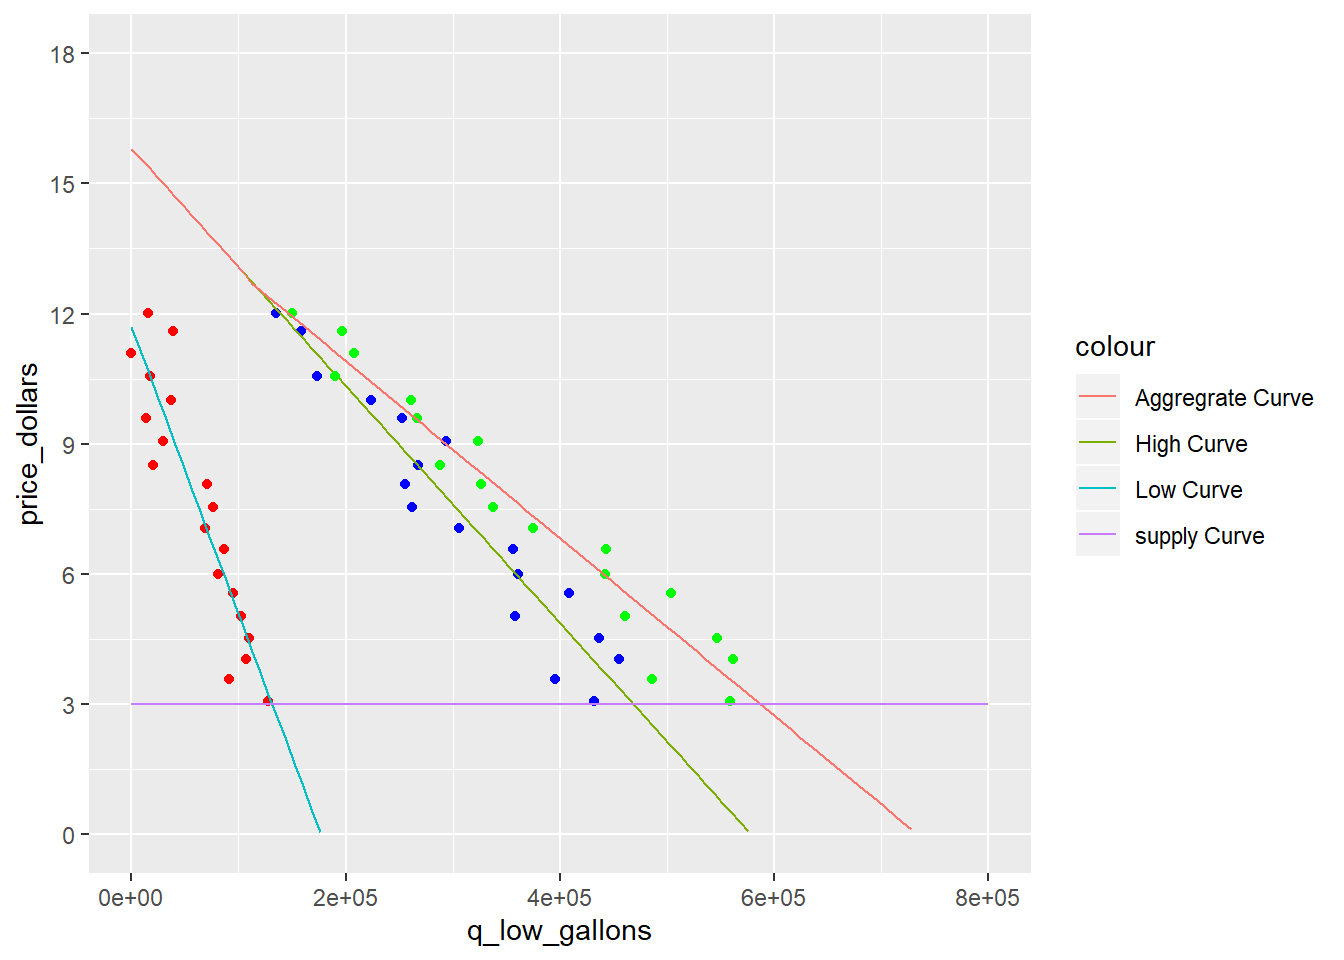
\includegraphics{assign_3_CF_AL_SA_files/figure-latex/plot_supply_demand-1.pdf}
1. Answer the following Questions:

\begin{enumerate}
\def\labelenumi{\alph{enumi}.}
\tightlist
\item
  What is the aggregate daily demand curve for gasoline?
\end{enumerate}

\(P=15.803\ensuremath{-2.731\times 10^{-5}}Q \text{ when }Q<106,119\)

\(P=15.002\ensuremath{-2.043\times 10^{-5}}Q\text{ when } Q\geq106,119\)

\begin{enumerate}
\def\labelenumi{\alph{enumi}.}
\setcounter{enumi}{1}
\tightlist
\item
  What is the supply curve for gasoline?
\end{enumerate}

\(P= \ensuremath{5.11\times 10^{-6}}Q\)

\begin{enumerate}
\def\labelenumi{\alph{enumi}.}
\setcounter{enumi}{2}
\tightlist
\item
  What is the ``benefit'' to consumers under the status quo?
\end{enumerate}

\begin{Shaded}
\begin{Highlighting}[]
\CommentTok{# find intersect of aggregate curve at P = $3.00 Q = 587482.43}
\NormalTok{agg_curve_intersect <-}\StringTok{ }\KeywordTok{uniroot}\NormalTok{(}\ControlFlowTok{function}\NormalTok{(q)\{}\KeywordTok{agg_demand}\NormalTok{(q)}\OperatorTok{-}\KeywordTok{supply}\NormalTok{(q)\},}\DataTypeTok{interval =} \KeywordTok{c}\NormalTok{(}\DecValTok{0}\NormalTok{,}\DecValTok{1}\NormalTok{),}\DataTypeTok{extendInt =} \StringTok{"yes"}\NormalTok{)}\OperatorTok{$}\NormalTok{root}

\CommentTok{# integrate to find total area under agg demand curve }
\NormalTok{gross_consumer_benefit <-}\StringTok{ }\KeywordTok{integrate}\NormalTok{(agg_demand,}\DataTypeTok{lower=}\DecValTok{0}\NormalTok{,}\DataTypeTok{upper=}\NormalTok{agg_curve_intersect)}\OperatorTok{$}\NormalTok{value}

\CommentTok{# integrate under the supply curve}
\NormalTok{producer_benefit <-}\StringTok{ }\KeywordTok{integrate}\NormalTok{(supply,}\DataTypeTok{lower=}\DecValTok{0}\NormalTok{,}\DataTypeTok{upper=}\NormalTok{agg_curve_intersect)}\OperatorTok{$}\NormalTok{value}
  
\CommentTok{# subtract gross_consumer and producer to find net consumer benefit}
\NormalTok{net_consumer_benefit <-}\StringTok{ }\NormalTok{gross_consumer_benefit }\OperatorTok{-}\StringTok{ }\NormalTok{producer_benefit}
\end{Highlighting}
\end{Shaded}

Consumer Benefit \(=\$5,334,270\)

\begin{enumerate}
\def\labelenumi{\alph{enumi}.}
\setcounter{enumi}{3}
\tightlist
\item
  What is the ``benefit'' to producers under the status quo?
\end{enumerate}

Producer Benefit \(=\$881,224\)

\begin{enumerate}
\def\labelenumi{\alph{enumi}.}
\setcounter{enumi}{4}
\tightlist
\item
  What is the environmental cost under the status quo (locally and in
  the rest of the world)?
\end{enumerate}

\begin{Shaded}
\begin{Highlighting}[]
\CommentTok{# integrate under each MEC from 0 to the agggrate curve intersect with supply curve}
\NormalTok{local_env_cost <-}\StringTok{ }\KeywordTok{integrate}\NormalTok{(local_env_cost_curve, }\DecValTok{0}\NormalTok{, agg_curve_intersect)}\OperatorTok{$}\NormalTok{value }\CommentTok{# 881223.6}
\NormalTok{global_env_cost <-}\StringTok{ }\KeywordTok{integrate}\NormalTok{(global_env_cost_curve, }\DecValTok{0}\NormalTok{, agg_curve_intersect)}\OperatorTok{$}\NormalTok{value }\CommentTok{# 293741.2}
\NormalTok{total_env_cost <-}\StringTok{  }\KeywordTok{integrate}\NormalTok{(total_env_cost_curve, }\DecValTok{0}\NormalTok{, agg_curve_intersect)}\OperatorTok{$}\NormalTok{value }\CommentTok{# 1174965}
\end{Highlighting}
\end{Shaded}

Local Environmental Cost \(=\$881,224\)

Global Environmental Cost \(=\$293,741\)

Total Environmental Cost \(=\$1,174,965\)

\begin{center}\rule{0.5\linewidth}{0.5pt}\end{center}

\begin{enumerate}
\def\labelenumi{\arabic{enumi}.}
\setcounter{enumi}{1}
\tightlist
\item
  How is the current consumer benefit divided between ``High'' and
  ``Low'' income consumers?
\end{enumerate}

\begin{Shaded}
\begin{Highlighting}[]
\NormalTok{high_curve_intersect <-}\StringTok{ }\KeywordTok{uniroot}\NormalTok{(}\ControlFlowTok{function}\NormalTok{(q)\{}\KeywordTok{high_demand}\NormalTok{(q)}\OperatorTok{-}\KeywordTok{supply}\NormalTok{(q)\},}\DataTypeTok{interval =} \KeywordTok{c}\NormalTok{(}\DecValTok{0}\NormalTok{,}\DecValTok{1}\NormalTok{),}\DataTypeTok{extendInt =} \StringTok{"yes"}\NormalTok{)}\OperatorTok{$}\NormalTok{root}
\NormalTok{low_curve_intersect <-}\StringTok{ }\KeywordTok{uniroot}\NormalTok{(}\ControlFlowTok{function}\NormalTok{(q)\{}\KeywordTok{low_demand}\NormalTok{(q)}\OperatorTok{-}\KeywordTok{supply}\NormalTok{(q)\},}\DataTypeTok{interval =} \KeywordTok{c}\NormalTok{(}\DecValTok{0}\NormalTok{,}\DecValTok{1}\NormalTok{),}\DataTypeTok{extendInt =} \StringTok{"yes"}\NormalTok{)}\OperatorTok{$}\NormalTok{root}

\NormalTok{high_gross_consumer_benefit <-}\StringTok{ }\KeywordTok{integrate}\NormalTok{(high_demand,}\DataTypeTok{lower=}\DecValTok{0}\NormalTok{,}\DataTypeTok{upper=}\NormalTok{high_curve_intersect)}\OperatorTok{$}\NormalTok{value}
\NormalTok{low_gross_consumer_benefit <-}\StringTok{ }\KeywordTok{integrate}\NormalTok{(low_demand,}\DataTypeTok{lower=}\DecValTok{0}\NormalTok{,}\DataTypeTok{upper=}\NormalTok{low_curve_intersect)}\OperatorTok{$}\NormalTok{value}
\end{Highlighting}
\end{Shaded}

High Consumer Benefit \(=\$4,459,118\)

Low Consumer Benefit \(=\$1,027,375\)

\begin{center}\rule{0.5\linewidth}{0.5pt}\end{center}

\begin{enumerate}
\def\labelenumi{\arabic{enumi}.}
\setcounter{enumi}{2}
\tightlist
\item
  A gas tax of \$1.00/gal. is proposed. What would be the effects of
  this tax on:
\end{enumerate}

\begin{enumerate}
\def\labelenumi{\alph{enumi}.}
\tightlist
\item
  The amount of gasoline produced and consumed.
\end{enumerate}

\begin{Shaded}
\begin{Highlighting}[]
\CommentTok{# Defining the tax rate}
\NormalTok{tax <-}\StringTok{ }\DecValTok{1}
\CommentTok{#functional supply curve with added tax}
\NormalTok{supply_tax <-}\StringTok{ }\ControlFlowTok{function}\NormalTok{(q)\{}\KeywordTok{supply}\NormalTok{(q)}\OperatorTok{+}\NormalTok{tax\}}

\CommentTok{#Agg curve intersect with new tax supply curve}
\NormalTok{agg_tax_curve_intersect <-}\StringTok{ }\KeywordTok{uniroot}\NormalTok{(}\ControlFlowTok{function}\NormalTok{(q)\{}\KeywordTok{agg_demand}\NormalTok{(q)}\OperatorTok{-}\KeywordTok{supply_tax}\NormalTok{(q)\},}\DataTypeTok{interval =} \KeywordTok{c}\NormalTok{(}\DecValTok{0}\NormalTok{,}\DecValTok{1}\NormalTok{),}\DataTypeTok{extendInt =} \StringTok{"yes"}\NormalTok{)}\OperatorTok{$}\NormalTok{root}
\end{Highlighting}
\end{Shaded}

Quantity Produced and consumed \(=548,323\)

\begin{enumerate}
\def\labelenumi{\alph{enumi}.}
\setcounter{enumi}{1}
\tightlist
\item
  The price of gasoline.
\end{enumerate}

\begin{Shaded}
\begin{Highlighting}[]
\NormalTok{tax_price <-}\StringTok{ }\KeywordTok{supply_tax}\NormalTok{(agg_tax_curve_intersect)}
\end{Highlighting}
\end{Shaded}

Quantity Produced and consumed \$=\(3.80\)

\begin{enumerate}
\def\labelenumi{\alph{enumi}.}
\setcounter{enumi}{2}
\tightlist
\item
  Welfare of ``High'' income consumers.
\end{enumerate}

\begin{Shaded}
\begin{Highlighting}[]
\CommentTok{# New curve intersects for high and low consumers}
\NormalTok{high_tax_curve_intersect <-}\StringTok{ }\KeywordTok{uniroot}\NormalTok{(}\ControlFlowTok{function}\NormalTok{(q)\{}\KeywordTok{high_demand}\NormalTok{(q)}\OperatorTok{-}\KeywordTok{supply_tax}\NormalTok{(q)\},}\DataTypeTok{interval =} \KeywordTok{c}\NormalTok{(}\DecValTok{0}\NormalTok{,}\DecValTok{1}\NormalTok{),}\DataTypeTok{extendInt =} \StringTok{"yes"}\NormalTok{)}\OperatorTok{$}\NormalTok{root}
\NormalTok{low_tax_curve_intersect <-}\StringTok{ }\KeywordTok{uniroot}\NormalTok{(}\ControlFlowTok{function}\NormalTok{(q)\{}\KeywordTok{low_demand}\NormalTok{(q)}\OperatorTok{-}\StringTok{  }\KeywordTok{supply_tax}\NormalTok{(q)\},}\DataTypeTok{interval =} \KeywordTok{c}\NormalTok{(}\DecValTok{0}\NormalTok{,}\DecValTok{1}\NormalTok{),}\DataTypeTok{extendInt =} \StringTok{"yes"}\NormalTok{)}\OperatorTok{$}\NormalTok{root}

\CommentTok{# Total consumer benefit under new tax paradigm}
\NormalTok{high_gross_consumer_welfare_tax <-}\StringTok{ }\KeywordTok{integrate}\NormalTok{(high_demand,}\DataTypeTok{lower=}\DecValTok{0}\NormalTok{,}\DataTypeTok{upper=}\NormalTok{high_tax_curve_intersect)}\OperatorTok{$}\NormalTok{value}
\NormalTok{low_gross_consumer_welfare_tax <-}\StringTok{ }\KeywordTok{integrate}\NormalTok{(low_demand,}\DataTypeTok{lower=}\DecValTok{0}\NormalTok{,}\DataTypeTok{upper=}\NormalTok{low_tax_curve_intersect)}\OperatorTok{$}\NormalTok{value}

\CommentTok{# Total Consumer taxes, incase the welfare is total benefit minus taxes...}
\NormalTok{high_tax_total <-}\StringTok{ }\NormalTok{high_tax_curve_intersect}
\NormalTok{low_tax_total <-}\StringTok{ }\NormalTok{low_tax_curve_intersect}
\end{Highlighting}
\end{Shaded}

High income consumer welfare \(=\$ 4,369,323\)

\begin{enumerate}
\def\labelenumi{\alph{enumi}.}
\setcounter{enumi}{3}
\tightlist
\item
  Welfare of ``Low'' income consumers.
\end{enumerate}

Low income consumer welfare \(\$ =1,009,094\)

\begin{enumerate}
\def\labelenumi{\alph{enumi}.}
\setcounter{enumi}{4}
\tightlist
\item
  Welfare of gas producers.
\end{enumerate}

\begin{Shaded}
\begin{Highlighting}[]
\CommentTok{# Producer welfare}
\NormalTok{producer_tax_welfare <-}\StringTok{ }\KeywordTok{integrate}\NormalTok{(supply,}\DataTypeTok{lower=}\DecValTok{0}\NormalTok{,}\DataTypeTok{upper=}\NormalTok{agg_tax_curve_intersect)}\OperatorTok{$}\NormalTok{value}
\end{Highlighting}
\end{Shaded}

Producer consumer welfare \(=\$ 767,659\)

\begin{enumerate}
\def\labelenumi{\alph{enumi}.}
\setcounter{enumi}{5}
\tightlist
\item
  Local environmental damage.
\end{enumerate}

\begin{Shaded}
\begin{Highlighting}[]
\CommentTok{# integrate under each MEC from 0 to the agggrate curve intersect with supply curve}
\NormalTok{local_env_cost_tax <-}\StringTok{ }\KeywordTok{integrate}\NormalTok{(local_env_cost_curve, }\DecValTok{0}\NormalTok{, agg_tax_curve_intersect)}\OperatorTok{$}\NormalTok{value }
\NormalTok{global_env_cost_tax <-}\StringTok{ }\KeywordTok{integrate}\NormalTok{(global_env_cost_curve, }\DecValTok{0}\NormalTok{, agg_tax_curve_intersect)}\OperatorTok{$}\NormalTok{value}
\NormalTok{total_env_cost_tax<-}\StringTok{  }\KeywordTok{integrate}\NormalTok{(total_env_cost_curve, }\DecValTok{0}\NormalTok{, agg_tax_curve_intersect)}\OperatorTok{$}\NormalTok{value }
\end{Highlighting}
\end{Shaded}

Local Environmental Cost with tax \(=\$822,484\)

\begin{enumerate}
\def\labelenumi{\alph{enumi}.}
\setcounter{enumi}{6}
\tightlist
\item
  Rest of world environmental damage.
\end{enumerate}

Global Environmental Cost with tax \(=\$274,161\)

\begin{enumerate}
\def\labelenumi{\alph{enumi}.}
\setcounter{enumi}{7}
\tightlist
\item
  Total revenue generated by the tax.
\end{enumerate}

\begin{Shaded}
\begin{Highlighting}[]
\CommentTok{# multiply the tax by the quantity produced}
\NormalTok{tax_revenue <-}\StringTok{ }\NormalTok{tax}\OperatorTok{*}\NormalTok{agg_tax_curve_intersect}
\end{Highlighting}
\end{Shaded}

Total tax revenue \(=\$548,323\)

\begin{center}\rule{0.5\linewidth}{0.5pt}\end{center}

\begin{enumerate}
\def\labelenumi{\arabic{enumi}.}
\setcounter{enumi}{3}
\tightlist
\item
  Now, assume that all revenue from a tax will be redistributed to the
  two groups in proportion to their pre-tax consumption of gas. For
  example, if 80\% of the gas was consumed by High income consumers,
  then they get 80\% of the tax revenue. Also assume that ``Low'' income
  consumers bear all local environmental costs. For a range of gas taxes
  (ranging from \$0 - \$5.00/gal), calculate the effects of the tax on:
\end{enumerate}

\begin{enumerate}
\def\labelenumi{\alph{enumi}.}
\tightlist
\item
  Overall welfare of ``High'' income consumers
\end{enumerate}

\begin{Shaded}
\begin{Highlighting}[]
\CommentTok{# The overall welfare consumers will change such that:}
\CommentTok{#   - the tax in proportion to pre-tax gas use is added to the welfare}
\CommentTok{#   - the local environmental cost for the tax based consumption is subtracted from the low income users}
\CommentTok{# To do this, we need to find:}
\CommentTok{#   - the proportion of gas consumption of high and low users}

\NormalTok{low_curve_intersect <-}\StringTok{ }\KeywordTok{uniroot}\NormalTok{(}\ControlFlowTok{function}\NormalTok{(q)\{}\KeywordTok{low_demand}\NormalTok{(q)}\OperatorTok{-}\KeywordTok{supply}\NormalTok{(q)\},}\DataTypeTok{interval =} \KeywordTok{c}\NormalTok{(}\DecValTok{0}\NormalTok{,}\DecValTok{1}\NormalTok{),}\DataTypeTok{extendInt =} \StringTok{"yes"}\NormalTok{)}\OperatorTok{$}\NormalTok{root}
\NormalTok{high_curve_intersect <-}\StringTok{ }\KeywordTok{uniroot}\NormalTok{(}\ControlFlowTok{function}\NormalTok{(q)\{}\KeywordTok{high_demand}\NormalTok{(q)}\OperatorTok{-}\KeywordTok{supply}\NormalTok{(q)\},}\DataTypeTok{interval =} \KeywordTok{c}\NormalTok{(}\DecValTok{0}\NormalTok{,}\DecValTok{1}\NormalTok{),}\DataTypeTok{extendInt =} \StringTok{"yes"}\NormalTok{)}\OperatorTok{$}\NormalTok{root}
\NormalTok{low_prop <-}\StringTok{ }\NormalTok{low_curve_intersect}\OperatorTok{/}\NormalTok{agg_curve_intersect }
\NormalTok{high_prop <-}\StringTok{ }\NormalTok{high_curve_intersect}\OperatorTok{/}\NormalTok{agg_curve_intersect }

\CommentTok{#   - the aggregate quantity consumed for a given tax rate to be used by finding local env cost}
\CommentTok{#   - the tax revenue for a given tax rate to find the tax redistribution}
\CommentTok{# }
\CommentTok{# To do this lets make a function where tax is the variable t. Then we will construct a dataframe }
\CommentTok{# which calculates between the range of 0-5, then we can plot it. We will need a function for both}
\CommentTok{# the high and low consumers}


\NormalTok{tax_fun <-}\StringTok{ }\ControlFlowTok{function}\NormalTok{(t) \{}
  
  \CommentTok{#find the new aggregate curve intersect based on the tax}
\NormalTok{  agg_tax_curve_intersect_var <-}\StringTok{ }\KeywordTok{uniroot}\NormalTok{(}\ControlFlowTok{function}\NormalTok{(q)\{}\KeywordTok{agg_demand}\NormalTok{(q)}\OperatorTok{-}\NormalTok{(}\KeywordTok{supply}\NormalTok{(q)}\OperatorTok{+}\NormalTok{t)\},}\DataTypeTok{interval =} \KeywordTok{c}\NormalTok{(}\DecValTok{0}\NormalTok{,}\DecValTok{1}\NormalTok{),}\DataTypeTok{extendInt =} \StringTok{"yes"}\NormalTok{)}\OperatorTok{$}\NormalTok{root}
\NormalTok{  high_tax_curve_intersect_var <-}\StringTok{ }\KeywordTok{uniroot}\NormalTok{(}\ControlFlowTok{function}\NormalTok{(q)\{}\KeywordTok{high_demand}\NormalTok{(q)}\OperatorTok{-}\NormalTok{(}\KeywordTok{supply}\NormalTok{(q)}\OperatorTok{+}\NormalTok{t)\},}\DataTypeTok{interval =} \KeywordTok{c}\NormalTok{(}\DecValTok{0}\NormalTok{,}\DecValTok{1}\NormalTok{),}\DataTypeTok{extendInt =} \StringTok{"yes"}\NormalTok{)}\OperatorTok{$}\NormalTok{root}
\NormalTok{  low_tax_curve_intersect_var <-}\StringTok{ }\KeywordTok{uniroot}\NormalTok{(}\ControlFlowTok{function}\NormalTok{(q)\{}\KeywordTok{low_demand}\NormalTok{(q)}\OperatorTok{-}\NormalTok{(}\KeywordTok{supply}\NormalTok{(q)}\OperatorTok{+}\NormalTok{t)\},}\DataTypeTok{interval =} \KeywordTok{c}\NormalTok{(}\DecValTok{0}\NormalTok{,}\DecValTok{1}\NormalTok{),}\DataTypeTok{extendInt =} \StringTok{"yes"}\NormalTok{)}\OperatorTok{$}\NormalTok{root}
  
  \CommentTok{#tax times the quantity}
\NormalTok{  total_tax_revenue <-}\StringTok{ }\NormalTok{t}\OperatorTok{*}\NormalTok{agg_tax_curve_intersect_var}
  
  \CommentTok{#redistribution of taxes}
\NormalTok{  redis_low <-}\StringTok{ }\NormalTok{low_prop }\OperatorTok{*}\StringTok{ }\NormalTok{total_tax_revenue}
\NormalTok{  redis_high <-}\StringTok{ }\NormalTok{high_prop }\OperatorTok{*}\StringTok{ }\NormalTok{total_tax_revenue}
  
\NormalTok{  local_env_cost_tax_var <-}\StringTok{ }\KeywordTok{integrate}\NormalTok{(local_env_cost_curve,}\DataTypeTok{lower=}\DecValTok{0}\NormalTok{,}\DataTypeTok{upper=}\NormalTok{agg_tax_curve_intersect_var)}\OperatorTok{$}\NormalTok{value}
  
\NormalTok{  high_welfare_var <-}\StringTok{ }\KeywordTok{integrate}\NormalTok{(high_demand,}\DataTypeTok{lower=}\DecValTok{0}\NormalTok{,}\DataTypeTok{upper=}\NormalTok{high_tax_curve_intersect_var)}\OperatorTok{$}\NormalTok{value }\OperatorTok{+}\StringTok{ }\NormalTok{redis_high}
\NormalTok{  low_welfare_var <-}\StringTok{ }\KeywordTok{integrate}\NormalTok{(low_demand,}\DataTypeTok{lower=}\DecValTok{0}\NormalTok{,}\DataTypeTok{upper=}\NormalTok{low_tax_curve_intersect_var)}\OperatorTok{$}\NormalTok{value }\OperatorTok{+}\NormalTok{redis_low }\OperatorTok{-}\NormalTok{local_env_cost_tax_var}
\NormalTok{  producer_welfare_var <-}\StringTok{ }\KeywordTok{integrate}\NormalTok{(supply,}\DataTypeTok{lower=}\DecValTok{0}\NormalTok{,}\DataTypeTok{upper=}\NormalTok{agg_tax_curve_intersect_var)}\OperatorTok{$}\NormalTok{value}
  
  \KeywordTok{return}\NormalTok{(}\KeywordTok{data.frame}\NormalTok{(}\DataTypeTok{tax=}\NormalTok{t,}\DataTypeTok{high_welfare =}\NormalTok{ high_welfare_var, }\DataTypeTok{low_welfare =}\NormalTok{ low_welfare_var, }\DataTypeTok{producer_welfare =}\NormalTok{ producer_welfare_var))}
    
\NormalTok{  \}}
  
\NormalTok{tax_df <-}\StringTok{ }\NormalTok{purrr}\OperatorTok{::}\KeywordTok{map_dfr}\NormalTok{(}\KeywordTok{seq}\NormalTok{(}\DataTypeTok{from=}\FloatTok{0.01}\NormalTok{,}\DataTypeTok{to=}\DecValTok{15}\NormalTok{,}\DataTypeTok{by=}\FloatTok{0.01}\NormalTok{),tax_fun)}
\end{Highlighting}
\end{Shaded}

\begin{Shaded}
\begin{Highlighting}[]
\KeywordTok{ggplot}\NormalTok{()}\OperatorTok{+}
\StringTok{  }\KeywordTok{geom_line}\NormalTok{(}\DataTypeTok{data=}\NormalTok{tax_df,}\KeywordTok{aes}\NormalTok{(}\DataTypeTok{x=}\NormalTok{tax,}\DataTypeTok{y=}\NormalTok{producer_welfare,}\DataTypeTok{color=}\StringTok{"Producer Welfare"}\NormalTok{))}\OperatorTok{+}
\StringTok{  }\KeywordTok{geom_line}\NormalTok{(}\DataTypeTok{data=}\NormalTok{tax_df,}\KeywordTok{aes}\NormalTok{(}\DataTypeTok{x=}\NormalTok{tax,}\DataTypeTok{y=}\NormalTok{high_welfare,}\DataTypeTok{color=}\StringTok{"High Welfare"}\NormalTok{))}\OperatorTok{+}
\StringTok{  }\KeywordTok{geom_line}\NormalTok{(}\DataTypeTok{data=}\NormalTok{tax_df,}\KeywordTok{aes}\NormalTok{(}\DataTypeTok{x=}\NormalTok{tax,}\DataTypeTok{y=}\NormalTok{low_welfare,}\DataTypeTok{color=}\StringTok{"Low Welfare"}\NormalTok{))}
\end{Highlighting}
\end{Shaded}

\includegraphics{assign_3_CF_AL_SA_files/figure-latex/unnamed-chunk-11-1.pdf}

\begin{enumerate}
\def\labelenumi{\alph{enumi}.}
\setcounter{enumi}{1}
\tightlist
\item
  Overall welfare of ``Low'' income consumers
\item
  Gas producers
\end{enumerate}

\begin{center}\rule{0.5\linewidth}{0.5pt}\end{center}

Simone

\begin{enumerate}
\def\labelenumi{\arabic{enumi}.}
\setcounter{enumi}{4}
\tightlist
\item
  A new electric car technology is invented and it lowers the demand
  curves of all income groups by half (vertically). Under these new
  demand curves, what are the effects on:
\end{enumerate}

\begin{Shaded}
\begin{Highlighting}[]
\CommentTok{# assert new demand curves divided by 50 vertically }
\NormalTok{I1_h<-}\StringTok{  }\NormalTok{lm_low}\OperatorTok{$}\NormalTok{coefficients[}\DecValTok{1}\NormalTok{]}\OperatorTok{/}\DecValTok{2}
\NormalTok{I2_h<-}\StringTok{  }\NormalTok{lm_high}\OperatorTok{$}\NormalTok{coefficients[}\DecValTok{1}\NormalTok{]}\OperatorTok{/}\DecValTok{2}

\NormalTok{low_demand_h <-}\StringTok{ }\ControlFlowTok{function}\NormalTok{(q)  I1_h }\OperatorTok{+}\StringTok{ }\NormalTok{S1}\OperatorTok{*}\NormalTok{q}
\NormalTok{high_demand_h<-}\StringTok{ }\ControlFlowTok{function}\NormalTok{(q) I2_h }\OperatorTok{+}\StringTok{ }\NormalTok{S2}\OperatorTok{*}\NormalTok{q}
\end{Highlighting}
\end{Shaded}

\begin{Shaded}
\begin{Highlighting}[]
\CommentTok{# Determines the 'dominate' curve for new curves. }
\NormalTok{demand_dom_h <-}\StringTok{ }\ControlFlowTok{function}\NormalTok{(q)\{}
  \ControlFlowTok{if}\NormalTok{ (I1_h}\OperatorTok{==}\NormalTok{I2_h)\{}\DecValTok{0}\NormalTok{\}}
  \ControlFlowTok{else} \ControlFlowTok{if}\NormalTok{(I1_h}\OperatorTok{>}\NormalTok{I2_h)\{}\KeywordTok{low_demand_h}\NormalTok{(q)\}}
  \ControlFlowTok{else} \ControlFlowTok{if}\NormalTok{(I2_h}\OperatorTok{>}\NormalTok{I1_h)\{}\KeywordTok{high_demand_h}\NormalTok{(q)\}}
\NormalTok{\}}
\CommentTok{# Determines q such that the new high demand and low demand are equal. #Used to find the kink in the curve. }
\NormalTok{intersect_point_h <-}\StringTok{ }\KeywordTok{abs}\NormalTok{(}\KeywordTok{uniroot}\NormalTok{(}\ControlFlowTok{function}\NormalTok{(q)\{}\KeywordTok{high_demand_h}\NormalTok{(q)}\OperatorTok{-}\KeywordTok{low_demand_h}\NormalTok{(q)\},}
                            \DataTypeTok{interval =} \KeywordTok{c}\NormalTok{(}\DecValTok{0}\NormalTok{,}\DecValTok{1}\NormalTok{),}\DataTypeTok{extendInt =} \StringTok{"yes"}\NormalTok{)}\OperatorTok{$}\NormalTok{root)}

\CommentTok{# functional defintion of new aggregate demand }
\CommentTok{# the function itself. When q is less than the interset, returns the 'dominant'}
\NormalTok{agg_demand_h <-}\StringTok{ }\ControlFlowTok{function}\NormalTok{(q) \{}\KeywordTok{ifelse}\NormalTok{(q}\OperatorTok{<}\NormalTok{intersect_point_h,}\KeywordTok{demand_dom_h}\NormalTok{(q),}
\NormalTok{                                  lm_agg}\OperatorTok{$}\NormalTok{coefficients[}\DecValTok{1}\NormalTok{]}\OperatorTok{/}\DecValTok{2} \OperatorTok{+}\StringTok{ }\NormalTok{(lm_agg}\OperatorTok{$}\NormalTok{coefficients[}\DecValTok{2}\NormalTok{]}\OperatorTok{*}\NormalTok{q))}
\NormalTok{\}}

\NormalTok{demand_dom_x_intersect_h <-}\StringTok{ }\KeywordTok{uniroot}\NormalTok{(demand_dom_h,}
                                  \DataTypeTok{interval =} \KeywordTok{c}\NormalTok{(}\DecValTok{0}\NormalTok{,}\DecValTok{1}\NormalTok{),}
                                  \DataTypeTok{extendInt =} \StringTok{"yes"}\NormalTok{)}\OperatorTok{$}\NormalTok{root}
\end{Highlighting}
\end{Shaded}

Aggregate Curve when Demand is decreased by 50\%

\(P=8\ensuremath{-2.7\times 10^{-5}}Q \text{ when }Q<53,059\)

\(P=8\ensuremath{-2\times 10^{-5}}Q\text{ when } Q\geq53,059\)

\begin{Shaded}
\begin{Highlighting}[]
\CommentTok{# find intersect of high & Low curves at P = $3.00 }
\NormalTok{high_curve_intersect_h <-}\StringTok{ }\KeywordTok{uniroot}\NormalTok{(}\ControlFlowTok{function}\NormalTok{(q)\{}\KeywordTok{high_demand_h}\NormalTok{(q)}\OperatorTok{-}\KeywordTok{supply}\NormalTok{(q)\},}\DataTypeTok{interval =} \KeywordTok{c}\NormalTok{(}\DecValTok{0}\NormalTok{,}\DecValTok{1}\NormalTok{),}\DataTypeTok{extendInt =} \StringTok{"yes"}\NormalTok{)}\OperatorTok{$}\NormalTok{root}

\NormalTok{low_curve_intersect_h <-}\StringTok{ }\KeywordTok{uniroot}\NormalTok{(}\ControlFlowTok{function}\NormalTok{(q)\{}\KeywordTok{low_demand_h}\NormalTok{(q)}\OperatorTok{-}\KeywordTok{supply}\NormalTok{(q)\},}\DataTypeTok{interval =} \KeywordTok{c}\NormalTok{(}\DecValTok{0}\NormalTok{,}\DecValTok{1}\NormalTok{),}\DataTypeTok{extendInt =} \StringTok{"yes"}\NormalTok{)}\OperatorTok{$}\NormalTok{root}
\end{Highlighting}
\end{Shaded}

\begin{enumerate}
\def\labelenumi{\alph{enumi}.}
\item
  Gas consumption by ``High'' income consumers \(=243,761\)
\item
  Gas consumption by ``Low'' income consumers \(=82,037\)
\item
  Gas price
\end{enumerate}

\begin{Shaded}
\begin{Highlighting}[]
\CommentTok{#New Agg curve intersect with supply curve P = 440637.96}
\NormalTok{agg_curve_intersect_h <-}\StringTok{ }\KeywordTok{uniroot}\NormalTok{(}\ControlFlowTok{function}\NormalTok{(q)\{}\KeywordTok{agg_demand_h}\NormalTok{(q)}\OperatorTok{-}\KeywordTok{supply}\NormalTok{(q)\},}\DataTypeTok{interval =} \KeywordTok{c}\NormalTok{(}\DecValTok{0}\NormalTok{,}\DecValTok{1}\NormalTok{),}\DataTypeTok{extendInt =} \StringTok{"yes"}\NormalTok{)}\OperatorTok{$}\NormalTok{root}
\end{Highlighting}
\end{Shaded}

\begin{Shaded}
\begin{Highlighting}[]
\CommentTok{# integrate under each MEC from 0 to the new agggrate curve intersect with supply curve}
\NormalTok{local_env_cost_h <-}\StringTok{ }\KeywordTok{integrate}\NormalTok{(local_env_cost_curve, }\DecValTok{0}\NormalTok{, agg_curve_intersect_h)}\OperatorTok{$}\NormalTok{value}

\NormalTok{global_env_cost_h <-}\StringTok{  }\KeywordTok{integrate}\NormalTok{(global_env_cost_curve, }\DecValTok{0}\NormalTok{, agg_curve_intersect_h)}\OperatorTok{$}\NormalTok{value }
\end{Highlighting}
\end{Shaded}

\begin{enumerate}
\def\labelenumi{\alph{enumi}.}
\setcounter{enumi}{3}
\item
  Local environmental damage from gasoline \(=440,612\)
\item
  Rest of world environmental damage from gasoline \(=146,871\)
\end{enumerate}

\begin{Shaded}
\begin{Highlighting}[]
\CommentTok{# Visualize}
\KeywordTok{ggplot}\NormalTok{()}\OperatorTok{+}
\StringTok{  }\KeywordTok{stat_function}\NormalTok{(}\KeywordTok{aes}\NormalTok{(}\DataTypeTok{x=}\DecValTok{0}\NormalTok{, }\DataTypeTok{color =} \StringTok{"Low Curve"}\NormalTok{), }\DataTypeTok{fun =}\NormalTok{ low_demand_h)}\OperatorTok{+}
\StringTok{  }\KeywordTok{stat_function}\NormalTok{(}\KeywordTok{aes}\NormalTok{(}\DataTypeTok{x=}\DecValTok{0}\NormalTok{, }\DataTypeTok{color =} \StringTok{"High Curve"}\NormalTok{), }\DataTypeTok{fun =}\NormalTok{ high_demand_h)}\OperatorTok{+}
\StringTok{  }\KeywordTok{stat_function}\NormalTok{(}\KeywordTok{aes}\NormalTok{(}\DataTypeTok{x=}\DecValTok{0}\NormalTok{, }\DataTypeTok{color =} \StringTok{"supply Curve"}\NormalTok{), }\DataTypeTok{fun =}\NormalTok{ supply)}\OperatorTok{+}\StringTok{ }\KeywordTok{stat_function}\NormalTok{(}\KeywordTok{aes}\NormalTok{(}\DataTypeTok{x=}\DecValTok{0}\NormalTok{, }\DataTypeTok{color =} \StringTok{"Aggregrate Curve"}\NormalTok{), }\DataTypeTok{fun =}\NormalTok{ agg_demand_h)}\OperatorTok{+}\StringTok{ }
\KeywordTok{xlim}\NormalTok{(}\DecValTok{0}\NormalTok{,}\DecValTok{400000}\NormalTok{)}\OperatorTok{+}\StringTok{ }
\StringTok{  }\KeywordTok{scale_y_continuous}\NormalTok{(}\DataTypeTok{breaks=}\KeywordTok{c}\NormalTok{(}\DecValTok{0}\NormalTok{,}\DecValTok{3}\NormalTok{,}\DecValTok{6}\NormalTok{,}\DecValTok{9}\NormalTok{,}\DecValTok{12}\NormalTok{,}\DecValTok{15}\NormalTok{,}\DecValTok{18}\NormalTok{),}\DataTypeTok{limits =} \KeywordTok{c}\NormalTok{(}\DecValTok{0}\NormalTok{,}\DecValTok{10}\NormalTok{))}
\end{Highlighting}
\end{Shaded}

\includegraphics{assign_3_CF_AL_SA_files/figure-latex/unnamed-chunk-17-1.pdf}

\begin{center}\rule{0.5\linewidth}{0.5pt}\end{center}

\begin{enumerate}
\def\labelenumi{\arabic{enumi}.}
\setcounter{enumi}{5}
\tightlist
\item
  Compare two situations:
\end{enumerate}

\begin{enumerate}
\def\labelenumi{\alph{enumi}.}
\item
  Total quantity of gasoline consumed with gas tax of \$1/gal. but no
  electric car technology\(=`rcomma(agg_tax_curve_intersect)`\)
\item
  Total quantity of gasoline consumed with no gas tax but with electric
  car technology\(=`rcomma(agg_curve_intersect_h)`\)
\end{enumerate}

\begin{Shaded}
\begin{Highlighting}[]
\NormalTok{consumption_difference<-}\StringTok{ }\NormalTok{agg_curve_intersect_h }\OperatorTok{-}\StringTok{ }\NormalTok{agg_curve_intersect}
\CommentTok{# intercept w/ electric cars = 293,741; is smaller than intercept without electric cars}
\end{Highlighting}
\end{Shaded}

Determine what value of tax makes the local environmental quality equal
between these two situations. Or in other words, what tax will lower the
Q* for the no electric cars scenario to the Q* in the electric car
scenario. When the quantity consumer is the same, the environmental cost
will also be equal.

\begin{Shaded}
\begin{Highlighting}[]
\CommentTok{# Find Price from no electric car aggregate curve when Q*= 293,741 electric car Q*}
\NormalTok{p_tax_increase <-}\StringTok{ }\KeywordTok{agg_demand}\NormalTok{(agg_curve_intersect_h) }
\end{Highlighting}
\end{Shaded}

\begin{Shaded}
\begin{Highlighting}[]
\CommentTok{# Solve p = supply()+ tax; for tax by rearranging now that we know our P* and Q* in the no electric cars scenario }
\NormalTok{increase_tax<-}\StringTok{ }\NormalTok{p_tax_increase}\OperatorTok{-}\StringTok{ }\NormalTok{supply_slope}\OperatorTok{*}\NormalTok{agg_curve_intersect_h}
\NormalTok{supply_increase_tax <-}\StringTok{ }\ControlFlowTok{function}\NormalTok{(q)\{}\KeywordTok{supply}\NormalTok{(q)}\OperatorTok{+}\NormalTok{increase_tax\}}

\CommentTok{#Agg curve intersect with adjusted tax supply curve}
\NormalTok{agg_tax_increase_curve_intersect <-}\StringTok{ }\KeywordTok{uniroot}\NormalTok{(}\ControlFlowTok{function}\NormalTok{(q)\{}\KeywordTok{agg_demand}\NormalTok{(q)}\OperatorTok{-}\KeywordTok{supply_increase_tax}\NormalTok{(q)\},}\DataTypeTok{interval =} \KeywordTok{c}\NormalTok{(}\DecValTok{0}\NormalTok{,}\DecValTok{1}\NormalTok{),}\DataTypeTok{extendInt =} \StringTok{"yes"}\NormalTok{)}\OperatorTok{$}\NormalTok{root}

\CommentTok{# Check that environmental cost is equal for both scenarios with new_tax}
\CommentTok{#Environmental Without electric cars + new tax }
\NormalTok{local_env_cost_increase_tax <-}\StringTok{ }\KeywordTok{integrate}\NormalTok{(local_env_cost_curve, }\DecValTok{0}\NormalTok{, agg_tax_increase_curve_intersect)}\OperatorTok{$}\NormalTok{value }

\CommentTok{# 440611.82}
\end{Highlighting}
\end{Shaded}

\begin{enumerate}
\def\labelenumi{\alph{enumi}.}
\setcounter{enumi}{3}
\item
  Local environmental damage from gasoline \(=440,612\)
\item
  Rest of world environmental damage from gasoline \(=146,871\)
\end{enumerate}

\begin{Shaded}
\begin{Highlighting}[]
\KeywordTok{ggplot}\NormalTok{()}\OperatorTok{+}
\StringTok{  }\KeywordTok{stat_function}\NormalTok{(}\KeywordTok{aes}\NormalTok{(}\DataTypeTok{x=}\DecValTok{0}\NormalTok{, }\DataTypeTok{color =} \StringTok{"Low Curve"}\NormalTok{), }\DataTypeTok{fun =}\NormalTok{ low_demand_h)}\OperatorTok{+}
\StringTok{  }\KeywordTok{stat_function}\NormalTok{(}\KeywordTok{aes}\NormalTok{(}\DataTypeTok{x=}\DecValTok{0}\NormalTok{, }\DataTypeTok{color =} \StringTok{"High Curve"}\NormalTok{), }\DataTypeTok{fun =}\NormalTok{ high_demand_h)}\OperatorTok{+}
\StringTok{  }\KeywordTok{stat_function}\NormalTok{(}\KeywordTok{aes}\NormalTok{(}\DataTypeTok{x=}\DecValTok{0}\NormalTok{, }\DataTypeTok{color =} \StringTok{"Supply Curve"}\NormalTok{), }\DataTypeTok{fun =}\NormalTok{ supply)}\OperatorTok{+}\StringTok{ }\KeywordTok{stat_function}\NormalTok{(}\KeywordTok{aes}\NormalTok{(}\DataTypeTok{x=}\DecValTok{0}\NormalTok{, }\DataTypeTok{color =} \StringTok{"Aggregrate Curve"}\NormalTok{), }\DataTypeTok{fun =}\NormalTok{ agg_demand_h)}\OperatorTok{+}\StringTok{ }
\KeywordTok{xlim}\NormalTok{(}\DecValTok{0}\NormalTok{,}\DecValTok{400000}\NormalTok{)}\OperatorTok{+}\StringTok{ }
\StringTok{  }\KeywordTok{scale_y_continuous}\NormalTok{(}\DataTypeTok{breaks=}\KeywordTok{c}\NormalTok{(}\DecValTok{0}\NormalTok{,}\DecValTok{3}\NormalTok{,}\DecValTok{6}\NormalTok{,}\DecValTok{9}\NormalTok{,}\DecValTok{12}\NormalTok{,}\DecValTok{15}\NormalTok{,}\DecValTok{18}\NormalTok{),}\DataTypeTok{limits =} \KeywordTok{c}\NormalTok{(}\DecValTok{0}\NormalTok{,}\DecValTok{10}\NormalTok{))}
\end{Highlighting}
\end{Shaded}

\includegraphics{assign_3_CF_AL_SA_files/figure-latex/unnamed-chunk-21-1.pdf}

\end{document}
